
%%--------------------------------------------------
%% Halliday: Fundamentals of Physics
%%--------------------------------------------------


%% Chapter 09: Center of Mass and Linear Momentum
%%--------------------------------------------------


%% Learning Objectives
%%--------------------------------------------------

%% 9.01: Given the positions of several particles along an axis or a plane, determine the location of their center of mass.
%% 9.02: Locate the center of mass of an extended, symmetric object by using the symmetry.
%% 9.03: For a two-dimensional or three-dimensional extended object with a uniform distribution of mass, determine the center of mass by (a) mentally dividing the object into simple geometric figures, each of which can be replaced by a particle at its center and (b) finding the center of mass of those particles.


%% Halliday Multiple Choice Questions
%%--------------------------------------------------
\element{halliday-mc}{
\begin{questionmult}{halliday-ch09-q01}
    Which one of the following statements is true?
    \begin{choices}
        \wrongchoice{the center of mass of an object must lie within the object}
        \wrongchoice{all the mass of an object is actually concentrated at its center of mass}
        \wrongchoice{the center of mass of an object cannot move if there is zero net force on the object}
        \wrongchoice{the center of mass of a cylinder must lie on its axis}
      %\correctchoice{none of the provided}
    \end{choices}
\end{questionmult}
}

\element{halliday-mc}{
\begin{question}{halliday-ch09-q02}
    The $x$ and $y$ coordinates of the center of mass of the three-particle system shown below are:
    \begin{center}
    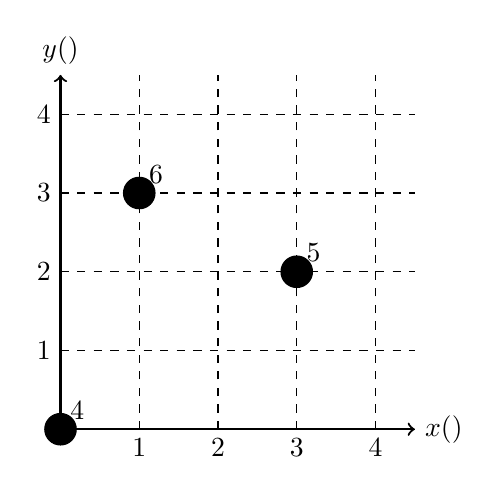
\begin{tikzpicture}
        %% Axis
        \draw[thick,->] (0,0) -- (0,4.5) node[pos=1.0,anchor=south] {$y(\si{\meter})$};
        \draw[thick,->] (0,0) -- (4.5,0) node[pos=1.0,anchor=west] {$x(\si{\meter})$};
        \foreach \x in {1,2,3,4} {
            \node[anchor=north] at (\x,0)  {\SI{\x}{\meter}};
            \node[anchor=east] at (0,\x)  {\SI{\x}{\meter}};
        }
        %% Grid
        \draw[dashed] (0,0) grid [step=1] (4.5,4.5);
        %% Masses
        \draw[fill] (0,0) circle (0.2) node[anchor=south west] {\SI{4}{\kilo\gram}};
        \draw[fill] (3,2) circle (0.2) node[anchor=south west] {\SI{5}{\kilo\gram}};
        \draw[fill] (1,3) circle (0.2) node[anchor=south west] {\SI{6}{\kilo\gram}};
    \end{tikzpicture}
    \end{center}
    \begin{multicols}{2}
    \begin{choices}
        \wrongchoice{zero, zero}
        \wrongchoice{\SI{1.3}{\meter}, \SI{1.7}{\meter}}
      \correctchoice{\SI{1.4}{\meter}, \SI{1.9}{\meter}}
        \wrongchoice{\SI{1.9}{\meter}, \SI{2.5}{\meter}}
        \wrongchoice{\SI{1.4}{\meter}, \SI{2.5}{\meter}}
    \end{choices}
    \end{multicols}
\end{question}
}

\element{halliday-mc}{
\begin{question}{halliday-ch09-q03}
    The center of mass of a uniform disk of radius $R$ is located:
    \begin{choices}
        \wrongchoice{on the rim}
        \wrongchoice{a distance $R/2$ from the center}
        \wrongchoice{a distance $R/3$ from the center}
        \wrongchoice{a distance $2R/3$ from the center}
      \correctchoice{at the center}
    \end{choices}
\end{question}
}

\element{halliday-mc}{
\begin{question}{halliday-ch09-q04}
    The center of mass of the system consisting of Earth,
        the Sun, and the planet Mars is:
    \begin{choices}
        \wrongchoice{closer to Earth than to either of the other bodies}
      \correctchoice{closer to the Sun than to either of the other bodies}
        \wrongchoice{closer to Mars than to either of the other bodies}
        \wrongchoice{at the geometric center of the triangle formed by the three bodies}
        \wrongchoice{at the center of the line joining Earth and Mars}
    \end{choices}
\end{question}
}

\element{halliday-mc}{
\begin{question}{halliday-ch09-q05}
    The center of mass of Earth's atmosphere is:
    \begin{choices}
        \wrongchoice{a little less than halfway between Earth's surface and the outer boundary of the atmosphere}
        \wrongchoice{near the surface of Earth}
        \wrongchoice{near the outer boundary of the atmosphere}
      \correctchoice{near the center of Earth}
        \wrongchoice{none of the provided}
    \end{choices}
\end{question}
}

\element{halliday-mc}{
\begin{question}{halliday-ch09-q06}
    A thick uniform wire is bent into the shape of the letter ``U'' as shown. 
    \begin{center}
    \begin{tikzpicture}
        %% Box
        \draw[line width=1pt] (-2,4) -- (-2,0) -- (2,0) -- (2,4);
        %% Labels
        \draw[fill] (-2,0) circle (2pt) node[anchor=north east] {$L$};
        \draw[fill] (0,0) circle (2pt) node[anchor=north] {$K$};
        \draw[fill] (0,1) circle (2pt) node[anchor=east] {$J$};
        \draw[fill] (0,2) circle (2pt) node[anchor=east] {$I$};
        \draw[fill] (2,0) circle (2pt) node[anchor=north west] {$M$};
    \end{tikzpicture}
    \end{center}
    Which point indicates the location of the center of mass of this wire?
    \begin{multicols}{5}
    \begin{choices}
        \wrongchoice{$I$}
      \correctchoice{$J$}
        \wrongchoice{$K$}
        \wrongchoice{$L$}
        \wrongchoice{$M$}
    \end{choices}
    \end{multicols}
\end{question}
}

\element{halliday-mc}{
\begin{question}{halliday-ch09-q07}
    A machinist starts with three identical square plates but cuts one corner from one of them,
        two corners from the second, and three corners from the third. 
    \begin{center}
    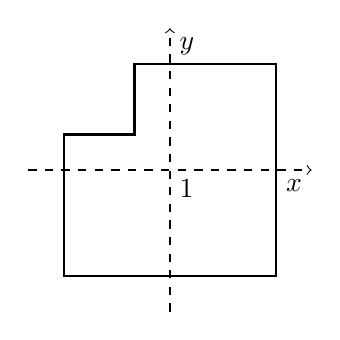
\begin{tikzpicture}[scale=0.9]
        \node[anchor=north west] at (0,0) {1};
        %% Axis
        \draw[dashed,->] (-2,0) -- (2,0) node[pos=1.0,anchor=north east] {$x$};
        \draw[dashed,->] (0,-2) -- (0,2) node[pos=1.0,anchor=north west] {$y$};
        %% Object
        \draw[thick] (-1.5,-1.5) -- (-1.5,0.5) -- (-0.5,0.5) -- (-0.5,1.5) -- (1.5,1.5) -- (1.5,-1.5) -- cycle;
    \end{tikzpicture}
    \hspace{1em}
    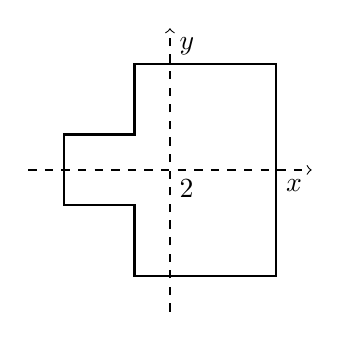
\begin{tikzpicture}[scale=0.9]
        \node[anchor=north west] at (0,0) {2};
        %% Axis
        \draw[dashed,->] (-2,0) -- (2,0) node[pos=1.0,anchor=north east] {$x$};
        \draw[dashed,->] (0,-2) -- (0,2) node[pos=1.0,anchor=north west] {$y$};
        %% Object
        \draw[thick] (-0.5,-1.5) -- (-0.5,-0.5) -- (-1.5,-0.5) -- (-1.5,0.5) -- (-0.5,0.5) -- (-0.5,1.5) -- (1.5,1.5) -- (1.5,-1.5) -- cycle;
    \end{tikzpicture}
    \hspace{1em}
    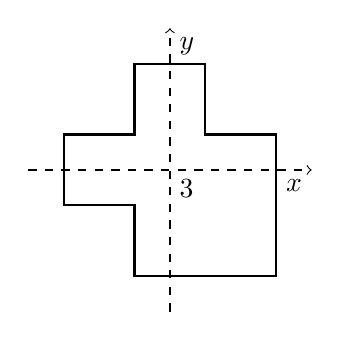
\begin{tikzpicture}[scale=0.9]
        \node[anchor=north west] at (0,0) {3};
        %% Axis
        \draw[dashed,->] (-2,0) -- (2,0) node[pos=1.0,anchor=north east] {$x$};
        \draw[dashed,->] (0,-2) -- (0,2) node[pos=1.0,anchor=north west] {$y$};
        %% Object
        \draw[thick] (-0.5,-1.5) -- (-0.5,-0.5) -- (-1.5,-0.5) -- (-1.5,0.5) -- (-0.5,0.5) -- (-0.5,1.5) -- (0.5,1.5) -- (0.5,0.5) -- (1.5,0.5) -- (1.5,-1.5) -- cycle;
    \end{tikzpicture}
    \end{center}
    Rank the three plates according to the $x$ coordinate of their centers of mass,
        from smallest to largest.
    \begin{multicols}{2}
    \begin{choices}
        \wrongchoice{1, 2, 3}
        \wrongchoice{1 and 2 tie, then 3}
        \wrongchoice{1, then 2 and 3 tie}
        \wrongchoice{3, 2, 1}
      \correctchoice{1 and 3 tie, then 2}
    \end{choices}
    \end{multicols}
\end{question}
}

\element{halliday-mc}{
\begin{question}{halliday-ch09-q08}
    Block $A$, with a mass of \SI{4}{\kilo\gram},
        is moving with a speed of \SI{2.0}{\meter\per\second} while block $B$,
        with a mass of \SI{8}{\kilo\gram},
        is moving in the opposite direction with a speed of \SI{3}{\meter\per\second}.
    The center of mass of the two block-system is moving with a velocity of:
    \begin{choices}
        \wrongchoice{\SI{1.3}{\meter\per\second} in the same direction as $A$}
      \correctchoice{\SI{1.3}{\meter\per\second} in the same direction as $B$}
        \wrongchoice{\SI{2.7}{\meter\per\second} in the same direction as $A$}
        \wrongchoice{\SI{1.0}{\meter\per\second} in the same direction as $B$}
        \wrongchoice{\SI{5.0}{\meter\per\second} in the same direction as $A$}
    \end{choices}
\end{question}
}

\element{halliday-mc}{
\begin{question}{halliday-ch09-q09}
    At the same instant that a \SI{0.50}{\kilo\gram} ball is dropped from \SI{25}{\meter} above Earth,
        a second ball, with a mass of \SI{0.25}{\kilo\gram},
        is thrown straight upward from Earth's surface with an initial speed of \SI{15}{\meter\per\second}.
    They move along nearby lines and pass each other without colliding. 
    At the end of \SI{2.0}{\second} the height above Earth's surface of the
        center of mass of the two-ball system is:
    \begin{multicols}{3}
    \begin{choices}
        \wrongchoice{\SI{2.9}{\meter}}
        \wrongchoice{\SI{4.0}{\meter}}
        \wrongchoice{\SI{5.0}{\meter}}
      \correctchoice{\SI{7.1}{\meter}}
        \wrongchoice{\SI{10.4}{\meter}}
    \end{choices}
    \end{multicols}
\end{question}
}

\element{halliday-mc}{
\begin{question}{halliday-ch09-q10}
    At the same instant that a \SI{0.50}{\kilo\gram} ball is dropped from \SI{25}{\meter} above Earth,
        a second ball, with a mass of \SI{0.25}{\kilo\gram},
        is thrown straight upward from Earth's surface with an initial speed of \SI{15}{\meter\per\second}.
    They move along nearby lines and pass without colliding. 
    At the end of \SI{2.0}{\second} the velocity of the center of mass of the two-ball system is:
    \begin{multicols}{2}
    \begin{choices}
        \wrongchoice{\SI{11}{\meter\per\second}, down}
        \wrongchoice{\SI{11}{\meter\per\second}, up}
      \correctchoice{\SI{15}{\meter\per\second}, down}
        \wrongchoice{\SI{15}{\meter\per\second}, up}
        \wrongchoice{\SI{20}{\meter\per\second}, down}
    \end{choices}
    \end{multicols}
\end{question}
}

\element{halliday-mc}{
\begin{question}{halliday-ch09-q11}
    At the same instant that a \SI{0.50}{\kilo\gram} ball is dropped from \SI{25}{\meter} above Earth,
        a second ball, with a mass of \SI{0.25}{\kilo\gram}, is thrown straight upward from Earth's surface with an initial speed of \SI{15}{\meter\per\second}.
    They move along nearby lines and pass without colliding. 
    At the end of \SI{2.0}{\second} the magnitude of the acceleration of the center of mass of the two-ball system is:
    \begin{multicols}{3}
    \begin{choices}
        \wrongchoice{$\dfrac{g}{4}$}
        \wrongchoice{$\dfrac{g}{2}$}
        \wrongchoice{$\dfrac{3g}{4}$}
      \correctchoice{$g$}
        \wrongchoice{$\dfrac{4g}{3}$}
    \end{choices}
    \end{multicols}
\end{question}
}

\element{halliday-mc}{
\begin{question}{halliday-ch09-q12}
    A light rope passes over a light frictionless pulley attached to the ceiling. 
    An object with a large mass is tied to one end and an object with a smaller mass is tied to one end and an object with a smaller mass is tied to the other end. 
    Starting from rest the heavier object moves downward and the lighter object moves upward with the same magnitude acceleration. 
    Which of the following statements is true for the system consisting of the two masses?
    \begin{choices}
        \wrongchoice{The center of mass remains at rest.}
        \wrongchoice{The net external force is zero.}
        \wrongchoice{The velocity of the center of mass is a constant.}
        \wrongchoice{The acceleration of the center of mass is $g$, downward.}
      \correctchoice{None of the provided statements are true.}
    \end{choices}
\end{question}
}

\element{halliday-mc}{
\begin{question}{halliday-ch09-q13}
    Two \SI{4.0}{\kilo\gram} blocks are tied together with a compressed spring between them. 
    They are thrown from the ground with an initial velocity of \SI{35}{\meter\per\second}, \ang{45} above the horizontal. 
    At the highest point of the trajectory they become untied and spring apart. 
    About how far below the highest point is the center of mass of the two-block system \SI{2.0}{\second} later,
        before either fragment has hit the ground?
    \begin{choices}
        \wrongchoice{\SI{12}{\meter}}
      \correctchoice{\SI{20}{\meter}}
        \wrongchoice{\SI{31}{\meter}}
        \wrongchoice{Can't tell because the velocities of the fragments are not given.}
        \wrongchoice{Can't tell because the coordinates of the highest point are not given.}
    \end{choices}
\end{question}
}

\element{halliday-mc}{
\begin{question}{halliday-ch09-q14}
    The center of mass of a system of particles has a constant velocity if:
    \begin{choices}
        \wrongchoice{the forces exerted by the particles on each other sum to zero}
      \correctchoice{the external forces acting on particles of the system sum to zero}
        \wrongchoice{the velocity of the center of mass is initially zero}
        \wrongchoice{the particles are distributed symmetrically around the center of mass}
        \wrongchoice{the center of mass is at the geometric center of the system}
    \end{choices}
\end{question}
}

\element{halliday-mc}{
\begin{question}{halliday-ch09-q15}
    The center of mass of a system of particles remains at the same place if:
    \begin{choices}
      \correctchoice{it is initially at rest and the external forces sum to zero}
        \wrongchoice{it is initially at rest and the internal forces sum to zero}
        \wrongchoice{the sum of the external forces is less than the maximum force of static friction}
        \wrongchoice{no friction acts internally}
        \wrongchoice{none of the provided}
    \end{choices}
\end{question}
}

\element{halliday-mc}{
\begin{question}{halliday-ch09-q16}
    A man sits in the back of a canoe in still water. 
    He then moves to the front of the canoe and sits there. 
    Afterwards the canoe:
    \begin{choices}
        \wrongchoice{is forward of its original position and moving forward}
        \wrongchoice{is forward of its original position and moving backward}
        \wrongchoice{is rearward of its original position and moving forward}
        \wrongchoice{is rearward of its original position and moving backward}
      \correctchoice{is rearward of its original position and not moving}
    \end{choices}
\end{question}
}

\element{halliday-mc}{
\begin{question}{halliday-ch09-q17}
    A \SI{640}{\newton} hunter gets a rope around a \SI{3200}{\newton} polar bear. 
    They are stationary, \SI{20}{\meter} apart,
        on frictionless level ice. 
    When the hunter pulls the polar bear to him,
        the polar bear will move:
    \begin{multicols}{3}
    \begin{choices}
        \wrongchoice{\SI{1.0}{\meter}}
      \correctchoice{\SI{3.3}{\meter}}
        \wrongchoice{\SI{10}{\meter}}
        \wrongchoice{\SI{12}{\meter}}
        \wrongchoice{\SI{17}{\meter}}
    \end{choices}
    \end{multicols}
\end{question}
}

\element{halliday-mc}{
\begin{question}{halliday-ch09-q18}
    Two boys, with masses of \SI{40}{\kilo\gram} and \SI{60}{\kilo\gram},
        respectively, stand on a horizontal frictionless surface holding the ends of a light \SI{10}{\meter} long rod. 
    The boys pull themselves together along the rod.
    When they meet the \SI{60}{\kilo\gram} boy will have moved what distance?
    \begin{multicols}{2}
    \begin{choices}
      \correctchoice{\SI{4}{\meter}}
        \wrongchoice{\SI{5}{\meter}}
        \wrongchoice{\SI{6}{\meter}}
        \wrongchoice{\SI{10}{\meter}}
        \wrongchoice{need to know the forces they exert}
    \end{choices}
    \end{multicols}
\end{question}
}

\element{halliday-mc}{
\begin{question}{halliday-ch09-q19}
    The center of mass of a system of particles obeys an equation similar to Newton's second law $\vec{F}=m\vec{a}_{com}$,
        where:
    \begin{choices}
        \wrongchoice{$\vec{F}$ is the net internal force and $m$ is the total mass of the system}
        \wrongchoice{$\vec{F}$ is the net internal force and $m$ is the mass acting on the system}
      \correctchoice{$\vec{F}$ is the net external force and $m$ is the total mass of the system}
        \wrongchoice{$\vec{F}$ is the force of gravity and $m$ is the mass of Earth}
        \wrongchoice{$\vec{F}$ is the force of gravity and $m$ is the total mass of the system}
    \end{choices}
\end{question}
}

\element{halliday-mc}{
\begin{question}{halliday-ch09-q20}
    A large wedge with a mass of 10 kg rests on a horizontal frictionless surface, as shown.
    A block with a mass of \SI{5.0}{\kilo\gram} starts from rest and slides down the inclined surface of the wedge,
        which is rough. 
    \begin{center}
    \begin{tikzpicture}
        %% Ground
        \draw (-1,0) -- (5,0);
        %% Ramp
        \draw (0,0) -- (4,3) -- (4,0) -- cycle;
        \node[anchor=center] at (3,1) {\SI{10}{\kilo\gram}};
        %% Ramp
        \node[anchor=south,rotate=36,draw,rectangle,minimum size=1cm] at (3,2.25) {\SI{5}{\kilo\gram}};
    \end{tikzpicture}
    \end{center}
    At one instant the vertical component of the block's velocity is \SI{3.0}{\meter\per\second} and the horizontal component is \SI{6.0}{\meter\per\second}. 
    At that instant the velocity of the wedge is:
    \begin{multicols}{2}
    \begin{choices}
        \wrongchoice{\SI{3.0}{\meter\per\second} to the left}
      \correctchoice{\SI{3.0}{\meter\per\second} to the right}
        \wrongchoice{\SI{6.0}{\meter\per\second} to the right}
        \wrongchoice{\SI{6.0}{\meter\per\second} to the left}
        \wrongchoice{\SI{17}{\meter\per\second} to the right}
    \end{choices}
    \end{multicols}
\end{question}
}

\element{halliday-mc}{
\begin{question}{halliday-ch09-q21}
    A \SI{2.0}{\kilo\gram} block is attached to one end of a spring with a spring constant of \SI{100}{\newton\per\meter} and a \SI{4.0}{\kilo\gram} block is attached to the other end.
    The blocks are placed on a horizontal frictionless surface and set into motion. 
    At one instant the \SI{2.0}{\kilo\gram} block is observed to be traveling to the right with a speed of 0.50 m/s and the 4.0-kg block is observed to be traveling to the left with a speed of \SI{0.30}{\meter\per\second}.
    Since the only forces on the blocks are the force of gravity,
        the normal force of the surface, and the force of the spring, we conclude that:
    \begin{choices}
        \wrongchoice{the spring is compressed at the time of the observation}
        \wrongchoice{the spring is not compressed at the time of observation}
        \wrongchoice{the motion was started with the masses at rest}
      \correctchoice{the motion was started with at least one of masses moving}
        \wrongchoice{the motion was started by compressing the spring}
    \end{choices}
\end{question}
}

\element{halliday-mc}{
\begin{question}{halliday-ch09-q22}
    A \SI{2.0}{\kilo\gram} mass is attached to one end of a spring with a spring constant of \SI{100}{\newton\per\meter} and a \SI{4.0}{\kilo\gram} mass is attached to the other end. 
    The masses are placed on a horizontal frictionless surface and the spring is compressed \SI{10}{\centi\meter}.
    The spring is then released with the masses at rest and the masses oscillate. 
    When the spring has its equilibrium length for the first time the \SI{2.0}{\kilo\gram} mass has a speed of 0.36 m/s. The mechanical energy that has been lost to the instant is:
    \begin{multicols}{3}
    \begin{choices}
        \wrongchoice{zero}
      \correctchoice{\SI{0.31}{\joule}}
        \wrongchoice{\SI{0.61}{\joule}}
        \wrongchoice{\SI{0.81}{\joule}}
        \wrongchoice{\SI{1.2}{\joule}}
    \end{choices}
    \end{multicols}
\end{question}
}

\element{halliday-mc}{
\begin{question}{halliday-ch09-q23}
    Momentum may be expressed in:
    \begin{choices}
        \wrongchoice{kilogram per meter (\si{\kilo\gram\per\meter})}
        \wrongchoice{gram second (\si{\gram\second})}
      \correctchoice{newton second (\si{\newton\second})}
        \wrongchoice{kilogram per meter per second (\si{\kilo\gram\per\meter\per\second})}
        \wrongchoice{newton per second (\si{\newton\per\second})}
    \end{choices}
\end{question}
}

\element{halliday-mc}{
\begin{question}{halliday-ch09-q24}
    The momentum of an object at a given instant is independent of its:
    \begin{multicols}{2}
    \begin{choices}
        \wrongchoice{inertia}
        \wrongchoice{mass}
        \wrongchoice{speed}
        \wrongchoice{velocity}
      \correctchoice{acceleration}
    \end{choices}
    \end{multicols}
\end{question}
}

\element{halliday-mc}{
\begin{question}{halliday-ch09-q25}
    Two bodies, $A$ and $B$, have equal kinetic energies. 
    The mass of $A$ is nine times that of $B$. 
    The ratio of the momentum of $A$ to that of $B$ is:
    \begin{multicols}{3}
    \begin{choices}
        \wrongchoice{$1:9$}
        \wrongchoice{$1:3$}
        \wrongchoice{$1:1$}
      \correctchoice{$3:1$}
        \wrongchoice{$9:1$}
    \end{choices}
    \end{multicols}
\end{question}
}

\element{halliday-mc}{
\begin{question}{halliday-ch09-q26}
    Two objects, $P$ and $Q$, have the same momentum. 
    $Q$ has more kinetic energy than $P$ if it:
    \begin{choices}
        \wrongchoice{weighs more than $P$}
      \correctchoice{is moving faster than $P$}
        \wrongchoice{weighs the same as $P$}
        \wrongchoice{is moving slower than $P$}
        \wrongchoice{is moving at the same speed as $P$}
    \end{choices}
\end{question}
}

\element{halliday-mc}{
\begin{question}{halliday-ch09-q27}
    A particle moves along the x axis. 
    Its momentum is graphed below as a function of time. 
    \begin{center}
    \begin{tikzpicture}
        %% Axis
        \draw (0,0) -- (0,3) node[anchor=east] {$p$};
        \draw (0,0) -- (5,0) node[anchor=north] {$t$};
        %% Line
        \draw (0,0.5) -- (1,2.5) node[pos=0.5,anchor=south east] {1}; %% 2
        \draw (1,2.5) -- (2,2.5) node[pos=0.5,anchor=south] {2}; %% 0
        \draw (2,2.5) -- (3,2) node[pos=0.5,anchor=south west] {3}; %%  0.5
        \draw (3,2) -- (4.5,0) node[pos=0.5,anchor=south west] {4}; %% 0.75
    \end{tikzpicture}
    \end{center}
    Rank the numbered regions according to the magnitude of the force acting on the particle,
        least to greatest.
    \begin{multicols}{2}
    \begin{choices}
        \wrongchoice{1, 2, 3, 4}
      \correctchoice{2, 3, 4, 1}
        \wrongchoice{1, 4, 3, 2}
        \wrongchoice{1, 3, 4, 2}
        \wrongchoice{2, 4, 3, 1}
    \end{choices}
    \end{multicols}
\end{question}
}

\element{halliday-mc}{
\begin{question}{halliday-ch09-q28}
    A \SI{1.0}{\kilo\gram} ball moving at \SI{2.0}{\meter\per\second} perpendicular to a wall rebounds from the wall at \SI{1.5}{\meter\per\second}.
    The change in the momentum of the ball is:
    \begin{choices}
        \wrongchoice{zero}
        \wrongchoice{\SI{0.5}{\newton\second} away from wall}
        \wrongchoice{\SI{0.5}{\newton\second} toward wall}
      \correctchoice{\SI{3.5}{\newton\second} away from wall}
        \wrongchoice{\SI{3.5}{\newton\second} toward wall}
    \end{choices}
\end{question}
}

\element{halliday-mc}{
\begin{question}{halliday-ch09-q29}
    If the total momentum of a system is changing:
    \begin{choices}
        \wrongchoice{particles of the system must be exerting forces on each other}
        \wrongchoice{the system must be under the influence of gravity}
        \wrongchoice{the center of mass must have constant velocity}
      \correctchoice{a net external force must be acting on the system}
        \wrongchoice{none of the provided}
    \end{choices}
\end{question}
}

\element{halliday-mc}{
\begin{question}{halliday-ch09-q30}
    When you step on the accelerator to increase the speed of your car,
        the force that accelerates the car is:
    \begin{choices}
        \wrongchoice{the force of your foot on the accelerator}
      \correctchoice{the force of friction of the road on the tires}
        \wrongchoice{the force of the engine on the drive shaft}
        \wrongchoice{the normal force of the road on the tires}
        \wrongchoice{none of the above}
    \end{choices}
\end{question}
}

\element{halliday-mc}{
\begin{question}{halliday-ch09-q31}
    A \SI{2.5}{\kilo\gram} stone is released from rest and falls toward Earth. 
    After \SI{4.0}{\second},
        the magnitude of its momentum is:
    \begin{multicols}{2}
    \begin{choices}
      \correctchoice{\SI{98}{\kilo\gram\meter\per\second}}
        \wrongchoice{\SI{78}{\kilo\gram\meter\per\second}}
        \wrongchoice{\SI{39}{\kilo\gram\meter\per\second}}
        \wrongchoice{\SI{24}{\kilo\gram\meter\per\second}}
        \wrongchoice{zero}
    \end{choices}
    \end{multicols}
\end{question}
}

\element{halliday-mc}{
\begin{question}{halliday-ch09-q32}
    A \SI{64}{\kilo\gram} woman stands on frictionless level ice with a \SI{0.10}{\kilo\gram} stone at her feet. 
    She kicks the stone with her foot so that she acquires a velocity of \SI{0.0017}{\meter\per\second} in the forward direction.
    The velocity acquired by the stone is:
    \begin{choices}
        \wrongchoice{\SI{1.1}{\meter\per\second} forward}
      \correctchoice{\SI{1.1}{\meter\per\second} backward}
        \wrongchoice{\SI{0.0017}{\meter\per\second} forward}
        \wrongchoice{\SI{0.0017}{\meter\per\second} backward}
        \wrongchoice{none of the provided}
    \end{choices}
\end{question}
}

\element{halliday-mc}{
\begin{question}{halliday-ch09-q33}
    A man is marooned at rest on level frictionless ice. 
    In desperation, he hurls his shoe to the right at \SI{15}{\meter\per\second}.
    If the man weighs \SI{720}{\newton} and the shoe weighs \SI{4.0}{\newton},
        the man moves to the left with a speed of:
    \begin{multicols}{2}
    \begin{choices}
        \wrongchoice{zero}
        \wrongchoice{\SI{2.1e-2}{\meter\per\second}}
      \correctchoice{\SI{8.3e-2}{\meter\per\second}}
        \wrongchoice{\SI{15}{\meter\per\second}}
        \wrongchoice{\SI{2.7e3}{\meter\per\second}}
    \end{choices}
    \end{multicols}
\end{question}
}

\element{halliday-mc}{
\begin{question}{halliday-ch09-q34}
    Two spacemen are floating together with zero speed in a gravity-free region of space. 
    The mass of spaceman $A$ is \SI{120}{\kilo\gram} and that of spaceman $B$ is \SI{90}{\kilo\gram}. 
    Spaceman $A$ pushes $B$ away from him with $B$ attaining a final speed of \SI{0.5}{\meter\per\second}.
    The final recoil speed of $A$ is:
    \begin{multicols}{3}
    \begin{choices}
        \wrongchoice{zero}
      \correctchoice{\SI{0.38}{\meter\per\second}}
        \wrongchoice{\SI{0.5}{\meter\per\second}}
        \wrongchoice{\SI{0.67}{\meter\per\second}}
        \wrongchoice{\SI{1.0}{\meter\per\second}}
    \end{choices}
    \end{multicols}
\end{question}
}

\element{halliday-mc}{
\begin{question}{halliday-ch09-q35}
    A projectile in flight explodes into several fragments. 
    The total momentum of the fragments immediately after this explosion:
    \begin{choices}
      \correctchoice{is the same as the momentum of the projectile immediately before the explosion}
        \wrongchoice{has been changed into kinetic energy of the fragments}
        \wrongchoice{is less than the momentum of the projectile immediately before the explosion}
        \wrongchoice{is more than the momentum of the projectile immediately before the explosion}
        \wrongchoice{has been changed into radiant energy}
    \end{choices}
\end{question}
}

\element{halliday-mc}{
\begin{question}{halliday-ch09-q36}
    A rifle of mass M is initially at rest but free to recoil. 
    It fires a bullet of mass m and velocity $v$ (relative to the ground). 
    After firing, the velocity of the rifle (relative to the ground) is:
    \begin{multicols}{3}
    \begin{choices}
        \wrongchoice{$-mv$}
        \wrongchoice{$-\dfrac{M v}{m}$}
      \correctchoice{$-\dfrac{m v}{M}$}
        \wrongchoice{$-v$}
        \wrongchoice{$\dfrac{m v}{M}$}
    \end{choices}
    \end{multicols}
\end{question}
}

\element{halliday-mc}{
\begin{question}{halliday-ch09-q37}
    Bullets from two revolvers are fired with the same velocity. 
    The bullet from gun \#1 is twice as heavy as the bullet from gun \#2. 
    Gun \#1 weighs three times as much as gun \#2. 
    The ratio of the momentum imparted to gun \#1 to that imparted to gun \#2 is:
    \begin{multicols}{3}
    \begin{choices}
        \wrongchoice{$2:3$}
        \wrongchoice{$3:2$}
      \correctchoice{$2:1$}
        \wrongchoice{$3:1$}
        \wrongchoice{$6:1$}
    \end{choices}
    \end{multicols}
\end{question}
}

\element{halliday-mc}{
\begin{question}{halliday-ch09-q38}
    A \SI{5}{\kilo\gram} object can move along the $x$ axis. 
    It is subjected to a force $F$ in the positive $x$ direction;
        a graph of $F$ as a function of time $t$ is shown below. 
    \begin{center}
    \begin{tikzpicture}
        \begin{axis}[
            axis y line=left,
            axis x line=bottom,
            axis line style={->},
            xlabel={time},
            x unit=\si{\second},
            xtick={1,2,3,4},
            ylabel={force},
            y unit=\si{\newton},
            ytick={2,4},
            xmin=0,xmax=4.5,
            ymin=0,ymax=4.5,
            width=0.8\columnwidth,
            height=0.5\columnwidth,
            very thin,
        ]
        \addplot[line width=1pt,mark=\empty] plot coordinates { (1,0) (2,4) (3,0) };
        \addplot[dashed,mark=\empty] plot coordinates { (0,4) (5,4) };
        \end{axis}
    \end{tikzpicture}
    \end{center}
    Over the time the force is applied the change in the velocity of the object is:
    \begin{multicols}{3}
    \begin{choices}
      \correctchoice{\SI{0.8}{\meter\per\second}}
        \wrongchoice{\SI{1.1}{\meter\per\second}}
        \wrongchoice{\SI{1.6}{\meter\per\second}}
        \wrongchoice{\SI{2.3}{\meter\per\second}}
        \wrongchoice{\SI{4.0}{\meter\per\second}}
    \end{choices}
    \end{multicols}
\end{question}
}

\element{halliday-mc}{
\begin{question}{halliday-ch09-q39}
    Force:
    \begin{choices}
        \wrongchoice{equals the negative integral (with respect to distance) of the potential energy function}
        \wrongchoice{is the ability to do work}
        \wrongchoice{is the rate of change of doing work}
      \correctchoice{equals the time rate of change of momentum}
        \wrongchoice{has dimensions of momentum multiplied by time}
    \end{choices}
\end{question}
}

\element{halliday-mc}{
\begin{question}{halliday-ch09-q40}
    Cart $A$, with a mass of \SI{0.20}{\kilo\gram},
        travels on a horizontal air track at \SI{3.0}{\meter\per\second} and hits cart $B$,
        which has a mass of \SI{0.40}{\kilo\gram} and is initially traveling away from $A$ at \SI{2.0}{\meter\per\second}.
    After the collision the center of mass of the two cart system has a speed of:
    \begin{multicols}{3}
    \begin{choices}
        \wrongchoice{zero}
      \correctchoice{\SI{0.33}{\meter\per\second}}
        \wrongchoice{\SI{2.3}{\meter\per\second}}
        \wrongchoice{\SI{2.5}{\meter\per\second}}
        \wrongchoice{\SI{5.0}{\meter\per\second}}
    \end{choices}
    \end{multicols}
\end{question}
}

\element{halliday-mc}{
\begin{question}{halliday-ch09-q41}
    A \SI{500}{\kilo\gram} sack of coal is dropped on a \SI{2000}{\kilo\gram} railroad flatcar which was initially moving at \SI{3}{\meter\per\second} as shown. 
    \begin{center}
    \begin{tikzpicture}
        %% Ground
        \node[anchor=north,fill,pattern=north east lines,minimum width=8cm, minimum height=0.05cm] at (-2,0) {};
        \draw (-6,0) -- (2,0);
        %% Flatbed
        \draw (-5,0.5) rectangle (0,1.0);
        \node[anchor=south east] at (0,0.5) {Santa Fe};
        \node[anchor=south west] at (-5,1) {\SI{2000}{\kilo\gram}};
        \draw[thick,->] (0,0.75) -- ++(0:1cm) node[pos=0.5,anchor=south] {\SI{3}{\meter\per\second}};
        %% Tires
        \draw (-5,0.5) -- (-4.5,0.15) -- (-4,0.15) -- (-3.5,0.5);
        \draw[fill=white] (-4.5,0.15) circle (0.15cm);
        \draw[fill=white] (-4.0,0.15) circle (0.15cm);
        \draw (0,0.5) -- (-0.5,0.15) -- (-1,0.15) -- (-1.5,0.5);
        \draw[fill=white] (-0.5,0.15) circle (0.15cm);
        \draw[fill=white] (-1.0,0.15) circle (0.15cm);
        %% Weight
        \node[anchor=south,fill,pattern=north east lines,minimum width=1cm, minimum height=0.05cm] at (1,4) {};
        \draw (0.5,4) -- (1.5,4);
        \node[draw,circle,fill=white!75!black,minimum size=2em] (A) at (1,3) {};
        \node[anchor=west] at (A.east) {\SI{500}{\kilo\gram}};
        \draw[thick] (A.north) -- (1,4);
    \end{tikzpicture}
    \end{center}
    After the sack rests on the flatcar,
        the speed of the flatcar is:
    \begin{multicols}{3}
    \begin{choices}
        \wrongchoice{\SI{0.6}{\meter\per\second}}
        \wrongchoice{\SI{1.2}{\meter\per\second}}
        \wrongchoice{\SI{1.8}{\meter\per\second}}
      \correctchoice{\SI{2.4}{\meter\per\second}}
        \wrongchoice{\SI{3.6}{\meter\per\second}}
    \end{choices}
    \end{multicols}
\end{question}
}

\element{halliday-mc}{
\begin{question}{halliday-ch09-q42}
    A cart loaded with sand slides forward along a horizontal frictionless track. 
    As the cart moves, sand trickles out at a constant rate through a hole in the back of the cart. 
    The acceleration of the cart is:
    \begin{choices}
        \wrongchoice{constant and in the forward direction}
        \wrongchoice{constant and in the backward direction}
        \wrongchoice{variable and in the forward direction}
        \wrongchoice{variable and in the backward direction}
      \correctchoice{zero}
    \end{choices}
\end{question}
}

\element{halliday-mc}{
\begin{question}{halliday-ch09-q43}
    The thrust of a rocket is:
    \begin{choices}
        \wrongchoice{a gravitational force acting on the rocket}
      \correctchoice{the force of the exiting fuel gases on the rocket}
        \wrongchoice{any force that is external to the rocket-fuel system}
        \wrongchoice{a force that arises from the reduction in mass of the rocket-fuel system}
        \wrongchoice{none of the provided}
    \end{choices}
\end{question}
}

\element{halliday-mc}{
\begin{question}{halliday-ch09-q44}
    At one instant of time a rocket is traveling in outer space at \SI{2500}{\meter\per\second} and is exhausting fuel at a rate of \SI{100}{\kilo\gram\per\second}. 
    If the speed of the fuel as it leaves the rocket is \SI{1500}{\meter\per\second},
        relative to the rocket, the thrust is:
    \begin{multicols}{2}
    \begin{choices}
        \wrongchoice{zero}
        \wrongchoice{\SI{1.0e5}{\newton}}
      \correctchoice{\SI{1.5e5}{\newton}}
        \wrongchoice{\SI{2.9e5}{\newton}}
        \wrongchoice{\SI{2.5e5}{\newton}}
    \end{choices}
    \end{multicols}
\end{question}
}

\element{halliday-mc}{
\begin{question}{halliday-ch09-q45}
    A rocket exhausts fuel with a velocity of \SI{1500}{\meter\per\second},
        relative to the rocket. 
    It starts from rest in outer space with fuel comprising \SI{80}{\percent} of the total mass. 
    When all the fuel has been exhausted its speed is:
    \begin{multicols}{2}
    \begin{choices}
        \wrongchoice{\SI{3600}{\meter\per\second}}
      \correctchoice{\SI{2400}{\meter\per\second}}
        \wrongchoice{\SI{1200}{\meter\per\second}}
        \wrongchoice{\SI{880}{\meter\per\second}}
        \wrongchoice{\SI{400}{\meter\per\second}}
    \end{choices}
    \end{multicols}
\end{question}
}

\element{halliday-mc}{
\begin{question}{halliday-ch09-q46}
    A \SI{1000}{\kilo\gram} space probe is motionless in space. 
    To start moving, its main engine is fired for \SI{5}{\second} during which time it ejects exhaust gases at \SI{5000}{\meter\per\second}. 
    \begin{center}
    \begin{tikzpicture}[yscale=0.8]
        %% Rocket
        \draw (0,1) to[out=180,in=90] (-2,0) to[out=270,in=180] (0,-1);
        \draw (0,1) -- (4,1);
        \draw (0,-1) -- (4,-1);
        \node[anchor=center] at (1,0) {\SI{1000}{\kilo\gram}};
        %% Fuel
        \draw (3.75,1) -- (3.75,0.50) to[out=45,in=180] (4.4,1);
        \draw (3.75,-1) -- (3.75,-0.50) to[out=345,in=180] (4.4,-1);
        \foreach \i in {5,15,25} {
            \draw (3,0) ++(\i:1) -- ++(\i:1.5);
            \draw (3,0) ++(-\i:1) -- ++(-\i:1.5);
        }
        %% Vectors
        \draw[thick,->] (1,-2) -- (0,-2) node[pos=0.5,anchor=south] {\SI{20}{\meter\per\second}};
        \draw[thick,->] (4,-2) -- (6,-2) node[pos=0.5,anchor=south] {\SI{5000}{\meter\per\second}};
    \end{tikzpicture}
    \end{center}
    At the end of this process it is moving at \SI{20}{\meter\per\second}. 
    The approximate mass of the ejected gas is:
    \begin{multicols}{3}
    \begin{choices}
        \wrongchoice{\SI{0.8}{\kilo\gram}}
      \correctchoice{\SI{4}{\kilo\gram}}
        \wrongchoice{\SI{5}{\kilo\gram}}
        \wrongchoice{\SI{20}{\kilo\gram}}
        \wrongchoice{\SI{25}{\kilo\gram}}
    \end{choices}
    \end{multicols}
\end{question}
}

\element{halliday-mc}{
\begin{question}{halliday-ch09-q47}
    The physical quantity ``impulse'' has the same dimensions as that of:
    \begin{multicols}{2}
    \begin{choices}
        \wrongchoice{force}
        \wrongchoice{power}
        \wrongchoice{energy}
      \correctchoice{momentum}
        \wrongchoice{work}
    \end{choices}
    \end{multicols}
\end{question}
}

\element{halliday-mc}{
\begin{question}{halliday-ch09-q48}
    The law of conservation of momentum applies to a system of colliding objects only if:
    \begin{choices}
        \wrongchoice{there is no change in kinetic energy of the system}
        \wrongchoice{the coefficient of restitution is one}
        \wrongchoice{the coefficient of restitution is zero}
      \correctchoice{the net external impulse is zero}
        \wrongchoice{the collisions are all elastic}
    \end{choices}
\end{question}
}

\element{halliday-mc}{
\begin{question}{halliday-ch09-q49}
    Sphere $X$, of mass \SI{2}{\kilo\gram}, is moving to the right at \SI{10}{\meter\per\second}.
    Sphere $Y$, of mass \SI{4}{\kilo\gram}, is moving to the left at \SI{10}{\meter\per\second}.
    The two spheres collide head-on. 
    The magnitude of the impulse of $X$ on $Y$ is:
    \begin{choices}
        \wrongchoice{twice the magnitude of the impulse of $Y$ on $X$}
        \wrongchoice{half the magnitude of the impulse of $Y$ on $X$}
        \wrongchoice{one-fourth the magnitude of the impulse of $Y$ on $X$}
        \wrongchoice{four times the magnitude of the impulse of $Y$ on $X$}
      \correctchoice{the same as the magnitude of the impulse of $Y$ on $X$}
    \end{choices}
\end{question}
}

\element{halliday-mc}{
\begin{question}{halliday-ch09-q50}
    Two bodies of unequal mass, placed at rest on a frictionless surface,
        are acted on by equal horizontal forces for equal times. 
    Just after these forces are removed,
        the body of greater mass will have:
    \begin{choices}
        \wrongchoice{the greater speed}
        \wrongchoice{the greater acceleration}
        \wrongchoice{the smaller momentum}
        \wrongchoice{the greater momentum}
      \correctchoice{the same momentum as the other body}
    \end{choices}
\end{question}
}

\element{halliday-mc}{
\begin{question}{halliday-ch09-q51}
    A \SI{0.2}{\kilo\gram} rubber ball is dropped from the window of a building. 
    It strikes the sidewalk below at \SI{30}{\meter\per\second} and rebounds up at \SI{20}{\meter\per\second}.
    The impulse on the ball during the collision is:
    \begin{multicols}{2}
    \begin{choices}
      \correctchoice{\SI{10}{\newton\second} upward}
        \wrongchoice{\SI{10}{\newton\second} downward}
        \wrongchoice{\SI{2.0}{\newton\second} upward}
        \wrongchoice{\SI{2.0}{\newton\second} downward}
        \wrongchoice{\SI{9.8}{\newton\second} upward}
    \end{choices}
    \end{multicols}
\end{question}
}

\element{halliday-mc}{
\begin{question}{halliday-ch09-q52}
    A \SI{10}{\kilo\gram} block of ice is at rest on a frictionless horizontal surface. 
    A \SI{1.0}{\newton} force is applied in an easterly direction for \SI{1.0}{\second}. 
    During this time interval, the block:
    \begin{choices}
        \wrongchoice{acquires a speed of \SI{1}{\meter\per\second}}
        \wrongchoice{moves \SI{10}{\centi\meter}}
      \correctchoice{acquires a momentum of \SI{1.0}{\kilo\gram\meter\per\second}}
        \wrongchoice{acquires a kinetic energy of \SI{0.1}{\joule}}
        \wrongchoice{none of the provided}
    \end{choices}
\end{question}
}

\element{halliday-mc}{
\begin{question}{halliday-ch09-q53}
    A uniform narrow bar, resting on ice,
        is given a transverse horizontal impulse $\vec{J}$ at one end as shown. 
    \begin{center}
    \begin{tikzpicture}[scale=0.8]
        \draw (-4,0) rectangle (4,1);
        \draw[fill] (0,0.5) circle (1.5pt) node[anchor=west] {COM};
        \draw[very thick,<-] (3,0) -- ++(270:1.5) node[pos=0.5,anchor=east] {$\vec{J}$};
    \end{tikzpicture}
    \end{center}
    The center of mass of the bar, COM, will then:
    \begin{choices}
        \wrongchoice{remain at rest}
        \wrongchoice{move in a circle}
      \correctchoice{move in a straight line}
        \wrongchoice{move in a parabola}
        \wrongchoice{move along some other curve}
    \end{choices}
\end{question}
}

\element{halliday-mc}{
\begin{question}{halliday-ch09-q54}
    What magnitude impulse will give a \SI{2.0}{\kilo\gram} object a momentum change of magnitude \SI{+50}{\kilo\gram\meter\per\second}?
    \begin{multicols}{3}
    \begin{choices}
        \wrongchoice{\SI{+25}{\newton\second}}
        \wrongchoice{\SI{-25}{\newton\second}}
      \correctchoice{\SI{+50}{\newton\second}}
        \wrongchoice{\SI{-50}{\newton\second}}
        \wrongchoice{\SI{+100}{\newton\second}}
    \end{choices}
    \end{multicols}
\end{question}
}

\element{halliday-mc}{
\begin{question}{halliday-ch09-q55}
    A student's life was saved in an automobile accident because an airbag expanded in front of his head. 
    If the car had not been equipped with an airbag,
        the windshield would have stopped the motion of his head in a much shorter time. 
    Compared to the windshield, the airbag:
    \begin{choices}
        \wrongchoice{causes a much smaller change in momentum}
        \wrongchoice{exerts a much smaller impulse}
        \wrongchoice{causes a much smaller change in kinetic energy}
      \correctchoice{exerts a much smaller force}
        \wrongchoice{does much more work}
    \end{choices}
\end{question}
}

\element{halliday-mc}{
\begin{question}{halliday-ch09-q56}
    A ball hits a wall and rebounds with the same speed, as diagramed below. 
    \begin{center}
    \begin{tikzpicture}
        %% Ground and axis label
        \draw (-3,0) -- (3,0) node[anchor=west] {$x$};
        \draw[dashed] (0,0) -- (0,3) node[anchor=east] {$y$};
        \node[anchor=north,fill,pattern=north east lines,minimum width=6cm, minimum height=0.05cm] at (0,0) {};
        %% Vectors
        \draw[very thick,->] (120:3) -- (120:0.1);
        \draw[very thick,->] (0,0) -- (60:3);
        %% Theta
        \draw[<->] (0,1.4) arc (90:120:1.4) node[pos=0.5,anchor=south] {$\theta$};
        \draw[<->] (0,1.6) arc (90:60:1.6) node[pos=0.5,anchor=south] {$\theta$};
    \end{tikzpicture}
    \end{center}
    The changes in the components of the momentum of the ball are:
    \begin{choices}
        \wrongchoice{$\Delta p_x > 0$, $\Delta p_y > 0$}
        \wrongchoice{$\Delta p_x < 0$, $\Delta p_y > 0$}
      \correctchoice{$\Delta p_x = 0$, $\Delta p_y > 0$}
        \wrongchoice{$\Delta p_x = 0$, $\Delta p_y < 0$}
        \wrongchoice{$\Delta p_x > 0$, $\Delta p_y < 0$}
    \end{choices}
\end{question}
}

\element{halliday-mc}{
\begin{question}{halliday-ch09-q57}
    A golf ball of mass $m$ is hit by a golf club so that the ball leaves the tee with speed $v$.
    The club is in contact with the ball for time $T$. 
    The magnitude of the average force on the club on the ball during the time $T$ is:
    \begin{multicols}{3}
    \begin{choices}
        \wrongchoice{$mvT$}
      \correctchoice{$\dfrac{mv}{T}$}
        \wrongchoice{$\dfrac{1}{2} mv^2 T$}
        \wrongchoice{$\dfrac{mv^2}{2T}$}
        \wrongchoice{$\dfrac{mT^2}{2v}$}
    \end{choices}
    \end{multicols}
\end{question}
}

\element{halliday-mc}{
\begin{question}{halliday-ch09-q58}
    A \SI{640}{\newton} acrobat falls \SI{5.0}{\meter} from rest into a net. 
    The net tosses him back up with the same speed he had just before he hit the net. 
    The magnitude of the average upward force exerted on him by the net during this collision is:
    \begin{choices}
        \wrongchoice{\SI{32}{\newton}}
        \wrongchoice{\SI{64}{\newton}}
        \wrongchoice{\SI{320}{\newton}}
        \wrongchoice{\SI{640}{\newton}}
      \correctchoice{impossible to determine from given data}
    \end{choices}
\end{question}
}

\element{halliday-mc}{
\begin{question}{halliday-ch09-q59}
    Whenever an object strikes a stationary object of equal mass:
    \begin{choices}
        \wrongchoice{the two objects cannot stick together}
        \wrongchoice{the collision must be elastic}
        \wrongchoice{the first object must stop}
        \wrongchoice{momentum is not necessarily conserved}
      \correctchoice{none of the provided}
    \end{choices}
\end{question}
}

\element{halliday-mc}{
\begin{question}{halliday-ch09-q60}
    For a two-body collision involving objects with different masses,
        a frame of reference which has the same velocity relative to the laboratory as does the center of mass of the two objects is:
    \begin{choices}
        \wrongchoice{a frame for which the momentum of the incident object is zero}
        \wrongchoice{a frame for which the momentum of the target object is zero}
        \wrongchoice{a frame for which the average momentum of the two objects is zero}
      \correctchoice{a frame for which the total momentum of the two objects is zero}
        \wrongchoice{none of the provided}
    \end{choices}
\end{question}
}

\element{halliday-mc}{
\begin{question}{halliday-ch09-q61}
    An inelastic collision is one in which:
    \begin{choices}
        \wrongchoice{momentum is not conserved but kinetic energy is conserved}
        \wrongchoice{total mass is not conserved but momentum is conserved}
        \wrongchoice{neither kinetic energy nor momentum is conserved}
      \correctchoice{momentum is conserved but kinetic energy is not conserved}
        \wrongchoice{the total impulse is equal to the change in kinetic energy}
    \end{choices}
\end{question}
}

\element{halliday-mc}{
\begin{question}{halliday-ch09-q62}
    A \SI{4.0}{\newton} puck is traveling at \SI{3.0}{\meter\per\second}.
    It strikes a \SI{8.0}{\newton} puck, which is stationary. 
    The two pucks stick together. 
    Their common final speed is:
    \begin{multicols}{3}
    \begin{choices}
      \correctchoice{\SI{1.0}{\meter\per\second}}
        \wrongchoice{\SI{1.5}{\meter\per\second}}
        \wrongchoice{\SI{2.0}{\meter\per\second}}
        \wrongchoice{\SI{2.3}{\meter\per\second}}
        \wrongchoice{\SI{3.0}{\meter\per\second}}
    \end{choices}
    \end{multicols}
\end{question}
}

\element{halliday-mc}{
\begin{question}{halliday-ch09-q63}
    A \SI{3.00}{\gram} bullet traveling horizontally at \SI{400}{\meter\per\second} hits a \SI{3.00}{\kilo\gram} wooden block,
        which is initially at rest on a smooth horizontal table. 
    The bullet buries itself in the block without passing through. 
    The speed of the block after the collision is:
    \begin{multicols}{3}
    \begin{choices}
        \wrongchoice{\SI{1.33}{\meter\per\second}}
      \correctchoice{\SI{0.40}{\meter\per\second}}
        \wrongchoice{\SI{12.0}{\meter\per\second}}
        \wrongchoice{\SI{40.0}{\meter\per\second}}
        \wrongchoice{\SI{160}{\meter\per\second}}
    \end{choices}
    \end{multicols}
\end{question}
}

\element{halliday-mc}{
\begin{question}{halliday-ch09-q64}
    A \SI{2}{\kilo\gram} cart, traveling on a horizontal air track with a speed of \SI{3}{\meter\per\second},
        collides with a stationary \SI{4}{\kilo\gram} cart. 
    The carts stick together. 
    The impulse exerted by one cart on the other has a magnitude of:
    \begin{multicols}{3}
    \begin{choices}
        \wrongchoice{zero}
      \correctchoice{\SI{4}{\newton\second}}
        \wrongchoice{\SI{6}{\newton\second}}
        \wrongchoice{\SI{9}{\newton\second}}
        \wrongchoice{\SI{12}{\newton\second}}
    \end{choices}
    \end{multicols}
\end{question}
}

\element{halliday-mc}{
\begin{question}{halliday-ch09-q65}
    A \SI{3}{\gram} bullet is fired horizontally into a \SI{10}{\kilo\gram} block of wood suspended by a rope from the ceiling. 
    The block swings in an arc,
        rising \SI{3}{\milli\meter} above its lowest position. 
    The velocity of the bullet was:
    \begin{choices}
        \wrongchoice{unknown since the heat generated in the collision was not given}
      \correctchoice{\SI{8.0e2}{\meter\per\second}}
        \wrongchoice{\SI{24.0}{\meter\per\second}}
        \wrongchoice{\SI{8.00}{\meter\per\second}}
        \wrongchoice{\SI{2.4e4}{\meter\per\second}}
    \end{choices}
\end{question}
}

\element{halliday-mc}{
\begin{question}{halliday-ch09-q66}
    A \SI{3.0}{\kilo\gram} and a \SI{2.0}{\kilo\gram} cart approach each other on a horizontal air track. 
    They collide and stick together. 
    After the collision their total kinetic energy is \SI{40}{\joule}. 
    The speed of their center of mass is:
    \begin{multicols}{2}
    \begin{choices}
        \wrongchoice{zero}
        \wrongchoice{\SI{2.8}{\meter\per\second}}
      \correctchoice{\SI{4.0}{\meter\per\second}}
        \wrongchoice{\SI{5.2}{\meter\per\second}}
        \wrongchoice{\SI{6.3}{\meter\per\second}}
    \end{choices}
    \end{multicols}
\end{question}
}

\element{halliday-mc}{
\begin{question}{halliday-ch09-q67}
    Blocks $A$ and $B$ are moving toward each other. 
    $A$ has a mass of \SI{2.0}{\kilo\gram} and a velocity of \SI{50}{\meter\per\second},
        while $B$ has a mass of \SI{4.0}{\kilo\gram} and a velocity of \SI{-25}{\meter\per\second}.
    They suffer a completely inelastic collision. 
    The kinetic energy lost during the collision is:
    \begin{multicols}{3}
    \begin{choices}
        \wrongchoice{zero}
        \wrongchoice{\SI{1250}{\joule}}
      \correctchoice{\SI{3750}{\joule}}
        \wrongchoice{\SI{5000}{\joule}}
        \wrongchoice{\SI{5600}{\joule}}
    \end{choices}
    \end{multicols}
\end{question}
}

\element{halliday-mc}{
\begin{question}{halliday-ch09-q68}
    For a completely inelastic two-body collision the kinetic energy retained by the objects is the same as:
    \begin{choices}
        \wrongchoice{the total kinetic energy before the collision}
        \wrongchoice{the difference in the kinetic energies of the objects before the collision}
      \correctchoice{$\dfrac{1}{2} M v_{com}^2$, where $M$ is the total mass and $v_{com}$ is the velocity of the center of mass}
        \wrongchoice{the kinetic energy of the more massive body before the collision}
        \wrongchoice{the kinetic energy of the less massive body before the collision}
    \end{choices}
\end{question}
}

\element{halliday-mc}{
\begin{question}{halliday-ch09-q69}
    A \SI{75}{\kilo\gram} man is riding in a \SI{30}{\kilo\gram} cart at \SI{2.0}{\meter\per\second}.
    He jumps off in such a way as to land on the ground with no horizontal velocity. 
    The resulting change in speed of the cart is:
    \begin{multicols}{3}
    \begin{choices}
        \wrongchoice{zero}
        \wrongchoice{\SI{2.0}{\meter\per\second}}
        \wrongchoice{\SI{3.0}{\meter\per\second}}
      \correctchoice{\SI{5.0}{\meter\per\second}}
        \wrongchoice{\SI{7.0}{\meter\per\second}}
    \end{choices}
    \end{multicols}
\end{question}
}

\element{halliday-mc}{
\begin{question}{halliday-ch09-q70}
    An elastic collision is one in which:
    \begin{choices}
        \wrongchoice{momentum is not conserved but kinetic energy is conserved}
        \wrongchoice{total mass is not conserved but momentum is conserved}
      \correctchoice{kinetic energy and momentum are both conserved}
        \wrongchoice{momentum is conserved but kinetic energy is not conserved}
        \wrongchoice{the total impulse is equal to the change in kinetic energy}
    \end{choices}
\end{question}
}

\element{halliday-mc}{
\begin{question}{halliday-ch09-q71}
    Object $A$ strikes the stationary object $B$ head-on in an elastic collision. 
    The mass of $A$ is fixed,
        you may choose the mass of $B$ appropriately. 
    Then:
    \begin{choices}
        \wrongchoice{for $B$ to have the greatest recoil speed, choose $m_B = m_A$}
        \wrongchoice{for $B$ to have the greatest recoil momentum, choose $m_B  \ll m_A$}
        \wrongchoice{for $B$ to have the greatest recoil kinetic energy, choose $m_B \ll m_A$}
        \wrongchoice{for $B$ to have the least recoil speed, choose $m_B = m_A$}
      \correctchoice{for $B$ to have the greatest recoil kinetic energy, choose $m_B = m_A$}
    \end{choices}
\end{question}
}

\element{halliday-mc}{
\begin{question}{halliday-ch09-q72}
    Block $A$, with a mass of \SI{2.0}{\kilo\gram},
        moves along the $x$ axis with a velocity of \SI{5.0}{\meter\per\second} in the positive $x$ direction.
    It suffers an elastic collision with block $B$,
        initially at rest, and the blocks leave the collision along the $x$ axis. 
    If $B$ is much more massive than $A$, the speed of $A$ after the collision is:
    \begin{multicols}{3}
    \begin{choices}
        \wrongchoice{zero}
        \wrongchoice{\SI{+5.0}{\meter\per\second}}
      \correctchoice{\SI{-5.0}{\meter\per\second}}
        \wrongchoice{\SI{+10}{\meter\per\second}}
        \wrongchoice{\SI{-10}{\meter\per\second}}
    \end{choices}
    \end{multicols}
\end{question}
}

\element{halliday-mc}{
\begin{question}{halliday-ch09-q73}
    A very massive object traveling at \SI{10}{\meter\per\second} strikes a very light object,
        initially at rest, and the light object moves off in the direction of travel of the heavy object. 
    If the collision is elastic, the speed of the lighter object is:
    \begin{multicols}{2}
    \begin{choices}
        \wrongchoice{\SI{5.0}{\meter\per\second}}
        \wrongchoice{\SI{10}{\meter\per\second}}
        \wrongchoice{\SI{15}{\meter\per\second}}
      \correctchoice{\SI{20}{\meter\per\second}}
        \wrongchoice{Can't tell from the information given.}
    \end{choices}
    \end{multicols}
\end{question}
}

\element{halliday-mc}{
\begin{question}{halliday-ch09-q74}
    Sphere $A$ has mass $m$ and is moving with velocity $v$. 
    It makes a head-on elastic collision with a stationary sphere $B$ of mass $2m$. 
    After the collision their speeds ($v_A$ and $v_B$) are:
    \begin{multicols}{2}
    \begin{choices}
        \wrongchoice{zero, $\dfrac{v}{2}$}
      \correctchoice{$-\dfrac{v}{3}$, $\dfrac{2v}{3}$}
        \wrongchoice{$-v$, $v$}
        \wrongchoice{$-\dfrac{2v}{3}$, $\dfrac{v}{3}$}
        \wrongchoice{none of the provided}
    \end{choices}
    \end{multicols}
\end{question}
}

\element{halliday-mc}{
\begin{question}{halliday-ch09-q75}
    Blocks $A$ and $B$ are moving toward each other along the $x$ axis. 
    A has a mass of \SI{2.0}{\kilo\gram} and a velocity of \SI{50}{\meter\per\second},
        while $B$ has a mass of \SI{4.0}{\kilo\gram} and a velocity of \SI{-25}{\meter\per\second}.
    They suffer an elastic collision and move off along the $x$ axis. 
    The kinetic energy transferred from $A$ to $B$ during the collision is:
    \begin{multicols}{3}
    \begin{choices}
      \correctchoice{zero}
        \wrongchoice{\SI{2500}{\joule}}
        \wrongchoice{\SI{5000}{\joule}}
        \wrongchoice{\SI{7500}{\joule}}
        \wrongchoice{\SI{10000}{\joule}}
    \end{choices}
    \end{multicols}
\end{question}
}

\element{halliday-mc}{
\begin{question}{halliday-ch09-q76}
    When a particle suffers a head-on elastic collision with another particle,
        initially at rest, the greatest fraction of kinetic energy is transferred if:
    \begin{choices}
        \wrongchoice{the incident particle is initially traveling very fast}
        \wrongchoice{the incident particle is traveling very slowly}
        \wrongchoice{the incident particle is much more massive than the target particle}
        \wrongchoice{the incident particle is much less massive than the target particle}
      \correctchoice{the incident and target particle have the same mass}
    \end{choices}
\end{question}
}

\element{halliday-mc}{
\begin{question}{halliday-ch09-q77}
    Two objects, $X$ and $Y$,
        are held at rest on a horizontal frictionless surface and a spring is compressed between them. 
    %% NOTE: changed from 2/5 to 5/2
    The mass of $X$ is $\frac{5}{2}$ times the mass of $Y$. 
    Immediately after the spring is released,
        $X$ has a kinetic energy of \SI{50}{\joule} and $Y$ has a kinetic energy of:
    \begin{multicols}{3}
    \begin{choices}
        \wrongchoice{\SI{20}{\joule}}
        \wrongchoice{\SI{8}{\joule}}
        \wrongchoice{\SI{310}{\joule}}
      \correctchoice{\SI{125}{\joule}}
        \wrongchoice{\SI{50}{\joule}}
    \end{choices}
    \end{multicols}
\end{question}
}

\element{halliday-mc}{
\begin{question}{halliday-ch09-q78}
    Two carts ($A$ and $B$), having spring bumpers, collide as shown. 
    Cart $A$ has a mass of \SI{2}{\kilo\gram} and is initially moving to the right. 
    Cart $B$ has a mass of \SI{3}{\kilo\gram} and is initially stationary. 
    \begin{center}
    \begin{tikzpicture}
        %% Ground
        \draw (-4,0) -- (4,0);
        \node[anchor=north,fill,pattern=north east lines,minimum width=8cm, minimum height=0.05cm] at (0,0) {};
        %% Cart A
        \node[anchor=south,rectangle,draw,minimum width=2cm,minimum height=1cm] (A) at (-2.5,0.25) {$A$};
        \draw[fill=white] (-3,0.25) circle (0.25);
        \draw[fill=white] (-2,0.25) circle (0.25);
        \draw[thick,->] (-3,2) -- (-1,2);
        \draw[thick,decoration={aspect=0.2,segment length=1mm,amplitude=2mm,coil},decorate] (A.east) -- ++(0:0.75);
        %% Cart B
        \node[anchor=south,rectangle,draw,minimum width=2cm,minimum height=1cm] (B) at (2.5,0.25) {$B$};
        \draw[fill=white] (3,0.25) circle (0.25);
        \draw[fill=white] (2,0.25) circle (0.25);
        \draw[thick,decoration={aspect=0.2,segment length=1mm,amplitude=2mm,coil},decorate] (B.west) -- ++(180:0.75);
    \end{tikzpicture}
    \end{center}
    When the separation between the carts is a minimum:
    \begin{choices}
        \wrongchoice{cart $B$ is still at rest}
        \wrongchoice{cart $A$ has come to rest}
        \wrongchoice{the carts have the same momentum}
        \wrongchoice{the carts have the same kinetic energy}
      \correctchoice{the kinetic energy of the system is at a minimum}
    \end{choices}
\end{question}
}

\element{halliday-mc}{
\begin{question}{halliday-ch09-q79}
    Two identical carts travel at \SI{1}{\meter\per\second} in opposite directions on a common horizontal surface. 
    They collide head-on and are reported to rebound,
        each with a speed of \SI{2}{\meter\per\second}.
    Then:
    \begin{choices}
        \wrongchoice{momentum was not conserved; therefore, the report must be false}
      \correctchoice{if some other form of energy were changed to kinetic during the collision, the report could be true}
        \wrongchoice{if the collision were elastic, the report could be true}
        \wrongchoice{if friction were present, the report could be true}
        \wrongchoice{if the duration of the collision were long enough, the report could be true}
    \end{choices}
\end{question}
}

\element{halliday-mc}{
\begin{question}{halliday-ch09-q80}
    A block moves at \SI{5.0}{\meter\per\second} in the positive $x$ direction and hits an identical block,
        initially at rest. 
    A small amount of gunpowder had been placed on one of the blocks. 
    The explosion does not harm the blocks but it doubles their total kinetic energy. 
    After the explosion the blocks move along the $x$ axis and the incident block has a speed in of:
    \begin{multicols}{2}
    \begin{choices}
      \correctchoice{\SI{1.8}{\meter\per\second}}
        \wrongchoice{\SI{5.0}{\meter\per\second}}
        \wrongchoice{\SI{6.8}{\meter\per\second}}
        \wrongchoice{\SI{7.1}{\meter\per\second}}
        \wrongchoice{\SI{11.8}{\meter\per\second}}
    \end{choices}
    \end{multicols}
\end{question}
}

\element{halliday-mc}{
\begin{question}{halliday-ch09-q81}
    A stream of gas consists of $n$ molecules. 
    Each molecule has mass $m$ and speed $v$.
    The stream is reflected elastically from a rigid surface as shown. 
    \begin{center}
    \begin{tikzpicture}
        %% Ground
        \draw (-4,0) -- (4,0);
        \node[anchor=north,fill,pattern=north east lines,minimum width=8cm, minimum height=0.05cm] at (0,0) {};
        %% Balls
        \foreach \i in {0,1,2,3,4} {
            \node[fill,circle,minimum size=0.1cm,anchor=south] at (150:\i) {};
            \node[fill,circle,minimum size=0.1cm,anchor=south] at (30:\i) {};
        }
        %% Vectors
        \draw[thick,->] (-2,2) -- ++(330:1) node[pos=0.5,anchor=south west] {$\vec{v}$};
        \draw[thick,<-] (+2,2) -- ++(210:1) node[pos=0.5,anchor=south east] {$\vec{v}$};
        %% Angles
        \draw[<->] (2,0) arc (0:30:2) node[pos=0.5,anchor=west] {\ang{30}};
        \draw[<->] (-2,0) arc (180:150:2) node[pos=0.5,anchor=east] {\ang{30}};
    \end{tikzpicture}
    \end{center}
    The magnitude of the change in the total momentum of the stream is:
    \begin{multicols}{2}
    \begin{choices}
        \wrongchoice{$2mnv$}
      \correctchoice{$2mnv \sin\ang{30}$}
        \wrongchoice{$mnv \sin\ang{30}$}
        \wrongchoice{$mnv \cos\ang{30}$}
        \wrongchoice{$mn v$}
    \end{choices}
    \end{multicols}
\end{question}
}


\endinput


